\chapter{Aufgabenstellung}
\label{chap:task}


\includepdf[pages=-]{../appendix/24FS_IMVS17_Generalisierte_Auswahlkomponente_Kolibri.pdf}



\chapter{Neue Komponente – Bilder}
\label{chap:newImgs}

\graphicspath{ {./img/newComponent/} }
\import{../appendix}{newComponentImgs.tex}
\graphicspath{ {./img/} }



\chapter{Existierende Komponenten – Bilder}
\label{chap:existingImgs}


\section*{Select}
\graphicspath{ {./img/select/} }
\import{../appendix}{existingSelectImgs.tex}
\graphicspath{ {./img/} }

\clearpage
\section*{Datalist}
\graphicspath{ {./img/datalist/} }
\import{../appendix}{existingDatalistImgs.tex}
\graphicspath{ {./img/} }



\chapter{User Test für Programmierer}
\label{chap:userTestProgrammers}


\section*{Code}

\lstinputlisting[style = htmlcssjs, caption = \codestyle{userTesting.js}, label = code:userTestingJs]{../userTest/userTesting.js}
\lstinputlisting[style = htmlcssjs, caption = \codestyle{userTesting.html}, label = code:userTestingHtml]{../userTest/userTesting.html}
\lstinputlisting[style = htmlcssjs, caption = \codestyle{starter.js}, label = code:starterJs]{../userTest/starter.js}
\begin{lstlisting}[style = htmlcssjs, caption = \codestyle{dataService.js}, label = code:dataServiceJs]
export {
    getAllContinents,
    getCountries,
    getCountriesChDeAt,
    getRegionsByCountry,
    getRegionsByCountryChDeAt,
    getYearsByDecade,
    getDecades,
    getLunchTypes,
};

/** @type { (String) => String } */
const getAllContinents = () => [
    ...new Set(...allCountriesWithContinent.map((country) => country.continent)),
];

/** @type { (String) => String } */
const getCountries = (continent) =>
    allCountriesWithContinent
        .filter((e) => e.continent === continent || !continent)
        .map((country) => country.country);

/** @type { (String) => String } */
const getRegionsByCountry = (country) =>
    allRegionsWithCountry
        .filter((e) => e.country === country || !country)
        .map((region) => region.region).sort();

/** @type { (String) => String } */
const getCountriesChDeAt = () => ["Switzerland", "Germany", "Austria"];

/** @type { (String) => String } */
const getRegionsByCountryChDeAt = (country) =>
    allRegionsWithCountry
        .filter(
            (e) => e.country === country || (!country && ["CH", "DE", "AT"].includes(e.code))
        )
        .map((region) => region.region).sort();

/** @type { (String) => String } */
const getYearsByDecade = (decade) => {
    const decadeStart = decade?.slice(0, 3);
    const data = [...Array(90).keys()].map((e) => e + 1930 + "");
    return data.filter((e) => !decade || e.startsWith(decadeStart));
};

/** @type { (String) => String } */
const getDecades = () => [...Array(9).keys()].map((e) => e * 10 + 1930 + "'s");

/** @type { (String) => String } */
const getLunchTypes = () => ["all", "vegetarian", "vegan", "flexetarian", "gluten-free", "lactose-free"];

/* data tables for `allCountriesWithContinent` and `allRegionsWithCountry` */
/* Link: https://github.com/fhnw-ramonamarti/fhnw-ramonamarti.github.io/blob/main/ip6/userTest/dataService_old.js */
\end{lstlisting}


\section*{Resultate}
\noindent
\textbf{Siehst du irgendwo Verbesserungspotenzial?}

\noindent 
- Detail: numberOfColumns ist etwas "verbose" 
\\
- Doku: In der Code Doku von SelectComponent dürfte der Return Value besser beschrieben werden (welches Array Element ist was). 
Das wird erst in den Anwendungsbeispielen klar. 

Keyboard navigation. 
Using keyboard to narrow down possible categories/values (maybe fuzzy searching), 
otherwise it takes me longer to find something than compared to a standard dropdown, even if the list there is bigger. 

ich finde es etwas unintuitiv beim SelectComponent neben den offensichtlich verständlichen selectAttributes (label, name, numberOfColumns) noch ein Callback mitzugeben. 
ich hätte mir mehr beschreibung gewünscht wie ich die komponente verwenden muss. 
(ich musste eher danach suchen.)

Bessere Dokumentation war verwirrend (Code). 

Automatisches Schliessen der Komponente nach der Auswahl würde ich praktisch finden. 

Es würde helfen, wenn die Types im JSDOC spezifiziert wären und wenn die Library eingebunden wäre. 
Dann wäre die Dokumentation leichter auffindbar. 

War mir am Anfang nicht klar dass was SelectComponent() zurückgibt und ob das Input-element sowie dass label-element selbst erstellt werden soll. 
Danach war es intuitiv anzuwenden. 

 \\

\noindent
\textbf{Bemerkung}

ich persönlich hatte zu beginn schwierigkeiten zu verstehen wie das framework funktioniert. 
die beschreibung für die tasks (ab task2) sind zum teil etwas unklar 
\\
=> The value data is provided by the function `Service.getRegionsByCountry()`, 
the categories are provided by the function `Service.getCountries()` 
\\
=> RegionsByCountry muss man noch das Country mitgeben. 
Hätte in der beschreibung drinstehen können. 

Nitpicking: while I see why the component is imported from a URL for the user tests, it makes it hard to use on a spotty network. 

 \\

Isch s selectAttributes `numberOfColumns` wörklich nötig? 
Vo mir uus gseh, chönt mer `numberOfColumns` vo `serviceCallbacks.length` ableite...? 
\\ Ehr hend nah recht es performance Problem wenn d liste lang isch... 
Dur s implementiere vo Task 2.2 brucht d websiite ca. 5 sekunde zum lade (rein Javascript execution). 
Das liht ned ahm Javascript, sondern am HTML rendering sowiit ih gseh ha. 
Ha suscht nah e Performance Trace gmacht wo mer in Chrome chan drii lade ahhghänkt. 
\\ Isch betz speziell, dass `serviceCallbacks` array in vercherter reihefolg muen drii geh werde wies denne ahhzeigt wird... 
\\ Wenn mer 2 Kollone het, aber rechts ke uuswahl, de chan mer au nüt uuswähle... 
Ja isch z erwarte aber isch au ih de Demo vorhande 
\\ För mich isch ned immer klaar gsii, wenns nah meh optione unde oder obedraa het. 


\graphicspath{ {./img/userTests/} }
\begin{figure}[!p]
    \centering
    \begin{minipage}[b]{0.6\textwidth}
        \centering
        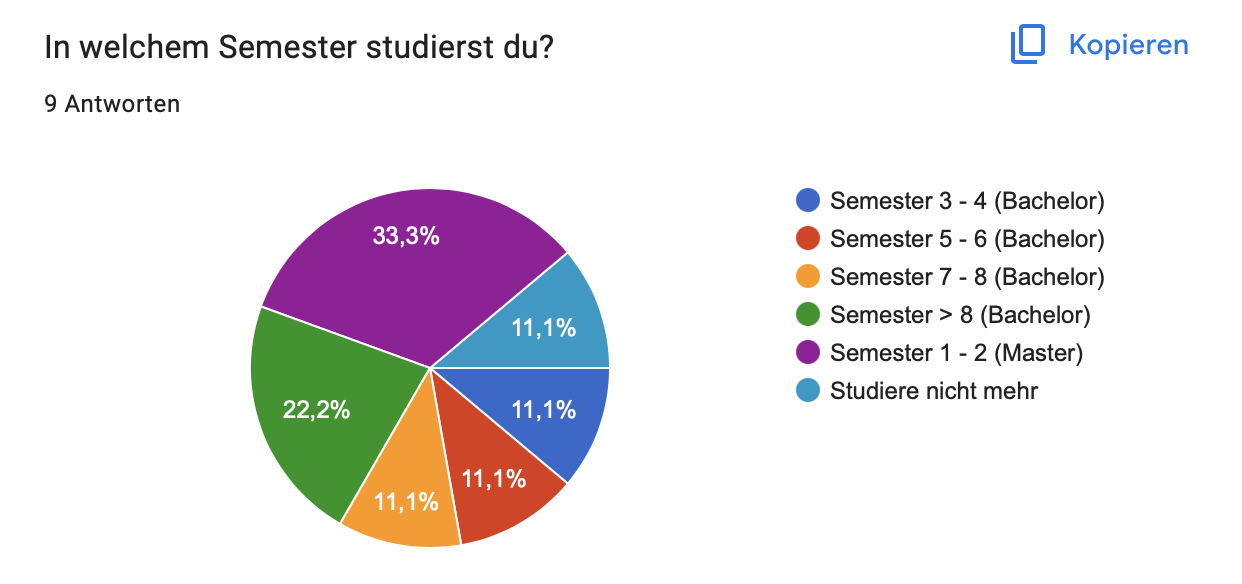
\includegraphics[width=\textwidth]{semester9.png}
        \caption{\centering User Test Programmierer Frage 1}
        \label{img:userTestSemester}
    \end{minipage}
    \begin{minipage}[b]{0.6\textwidth}
        \centering
        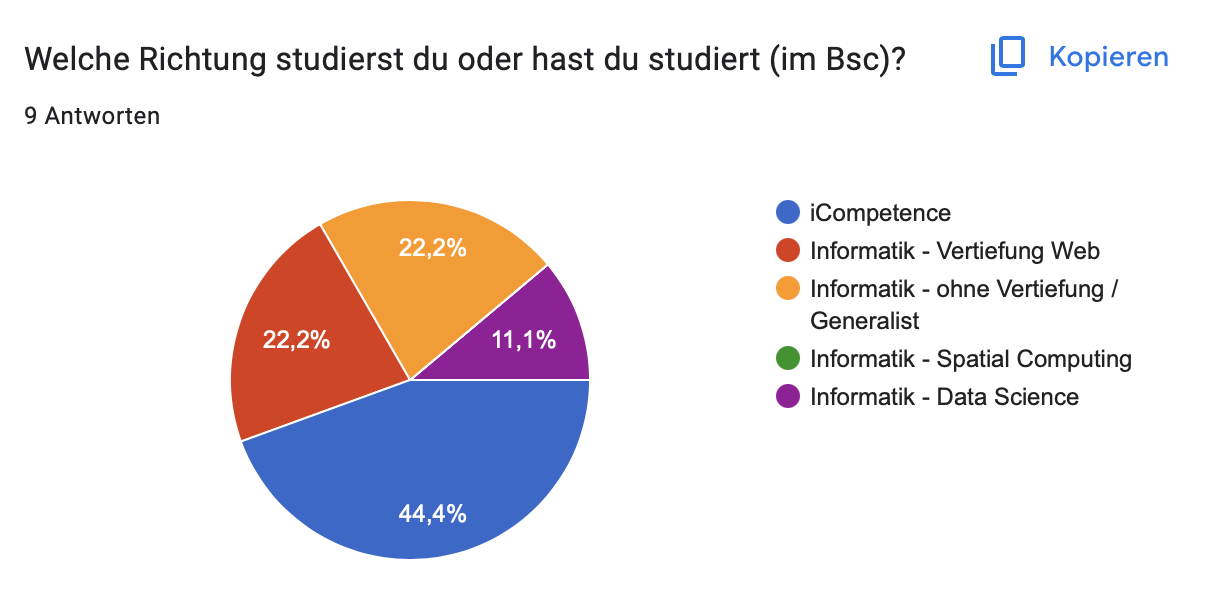
\includegraphics[width=\textwidth]{richtung9.png}
        \caption{\centering User Test Programmierer Frage 2}
        \label{img:userTestStudy}
    \end{minipage}
    \begin{minipage}[b]{0.6\textwidth}
        \centering
        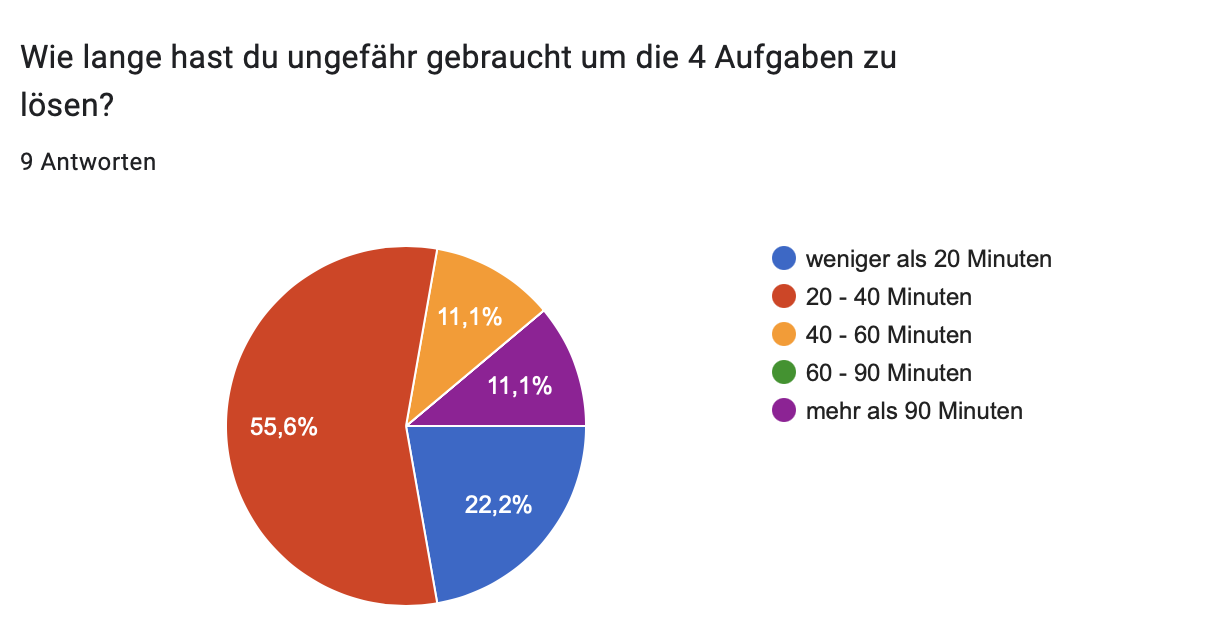
\includegraphics[width=\textwidth]{dauer9.png}
        \caption{\centering User Test Programmierer Frage 3}
        \label{img:userTestDuration}
    \end{minipage}
    \begin{minipage}[b]{0.6\textwidth}
        \centering
        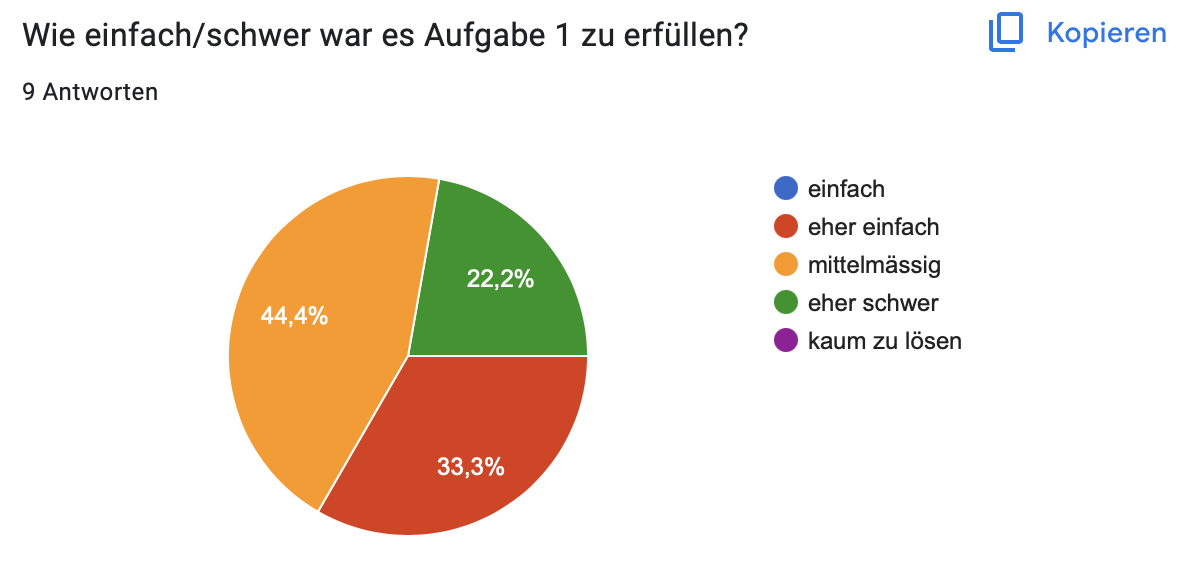
\includegraphics[width=\textwidth]{a1_9.png}
        \caption{\centering User Test Programmierer Frage 4}
        \label{img:userTestA1}
    \end{minipage}
\end{figure}

\begin{figure}[!p]
    \centering
    \begin{minipage}[b]{0.6\textwidth}
        \centering
        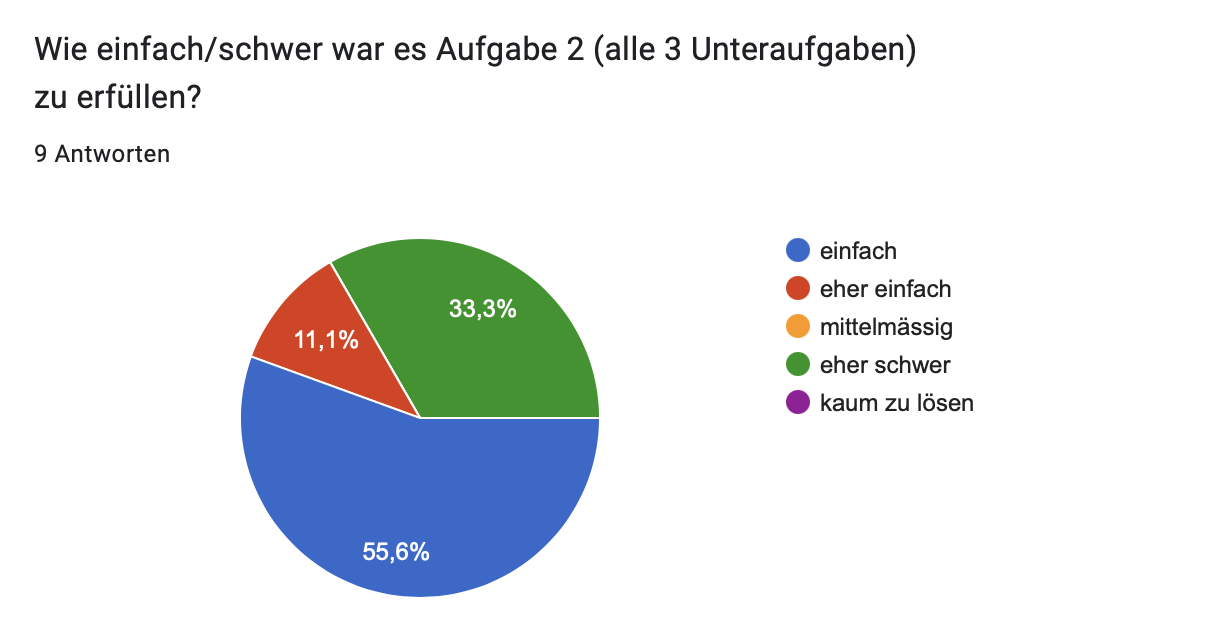
\includegraphics[width=\textwidth]{a2_9.png}
        \caption{\centering User Test Programmierer Frage 5}
        \label{img:userTestA2}
    \end{minipage}
    \begin{minipage}[b]{0.6\textwidth}
        \centering
        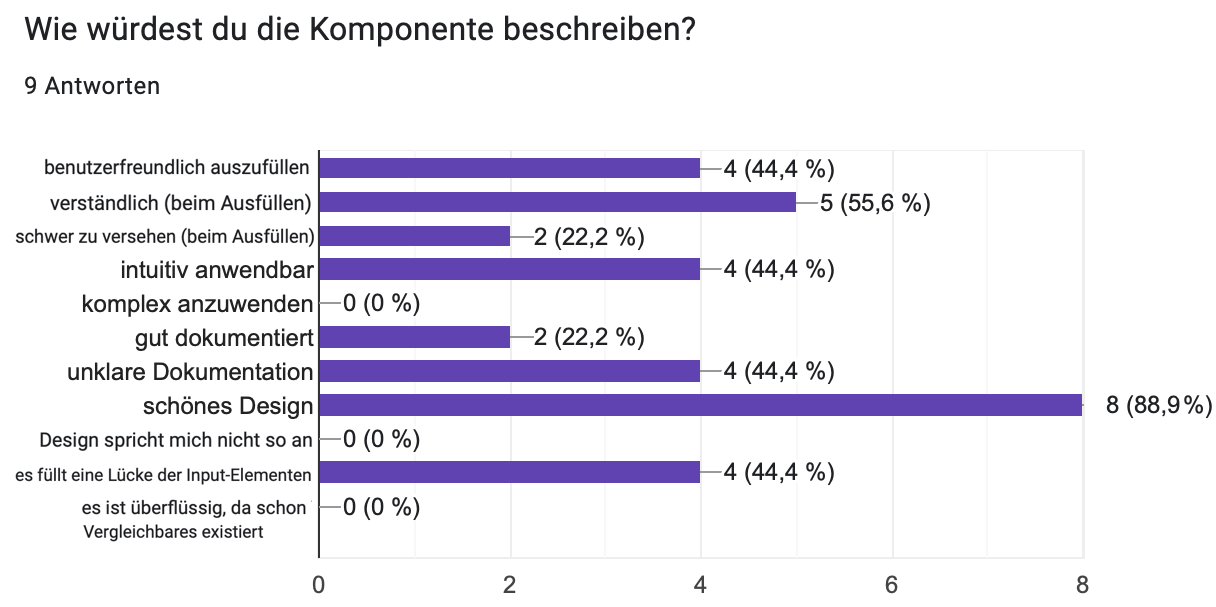
\includegraphics[width=\textwidth]{desc9.png}
        \caption{\centering User Test Programmierer Frage 6}
        \label{img:userTestDesc}
    \end{minipage}
    \begin{minipage}[b]{0.6\textwidth}
        \centering
        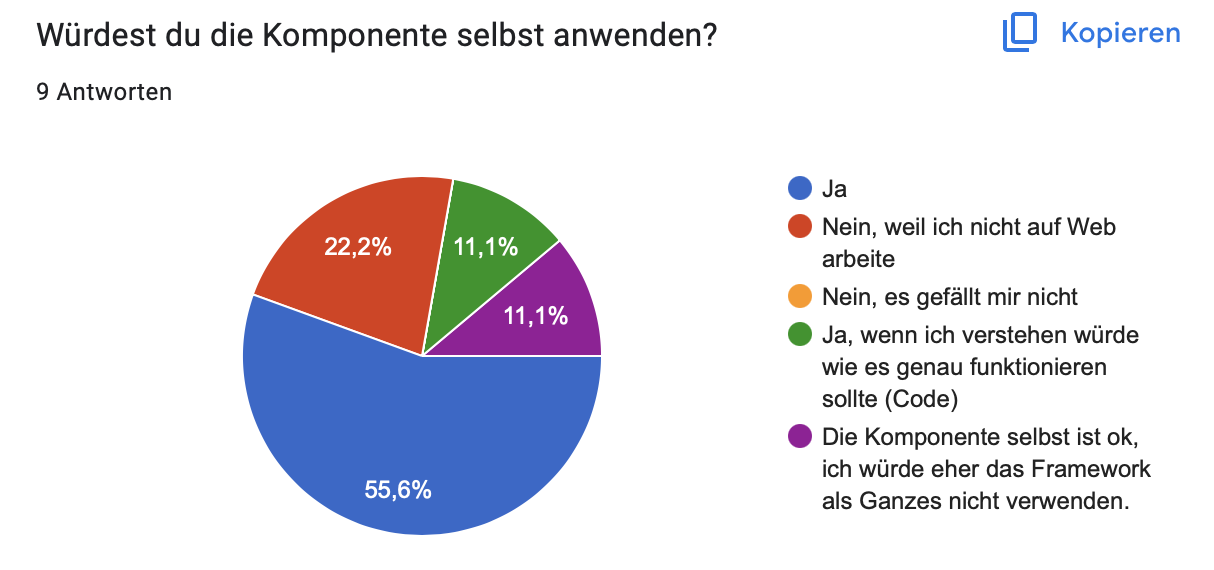
\includegraphics[width=\textwidth]{anwenden9.png}
        \caption{\centering User Test Programmierer Frage 7}
        \label{img:userTestUsage}
    \end{minipage}
\end{figure}
\graphicspath{ {./img/} }



\chapter{Personas}
\label{chap:perosnas}

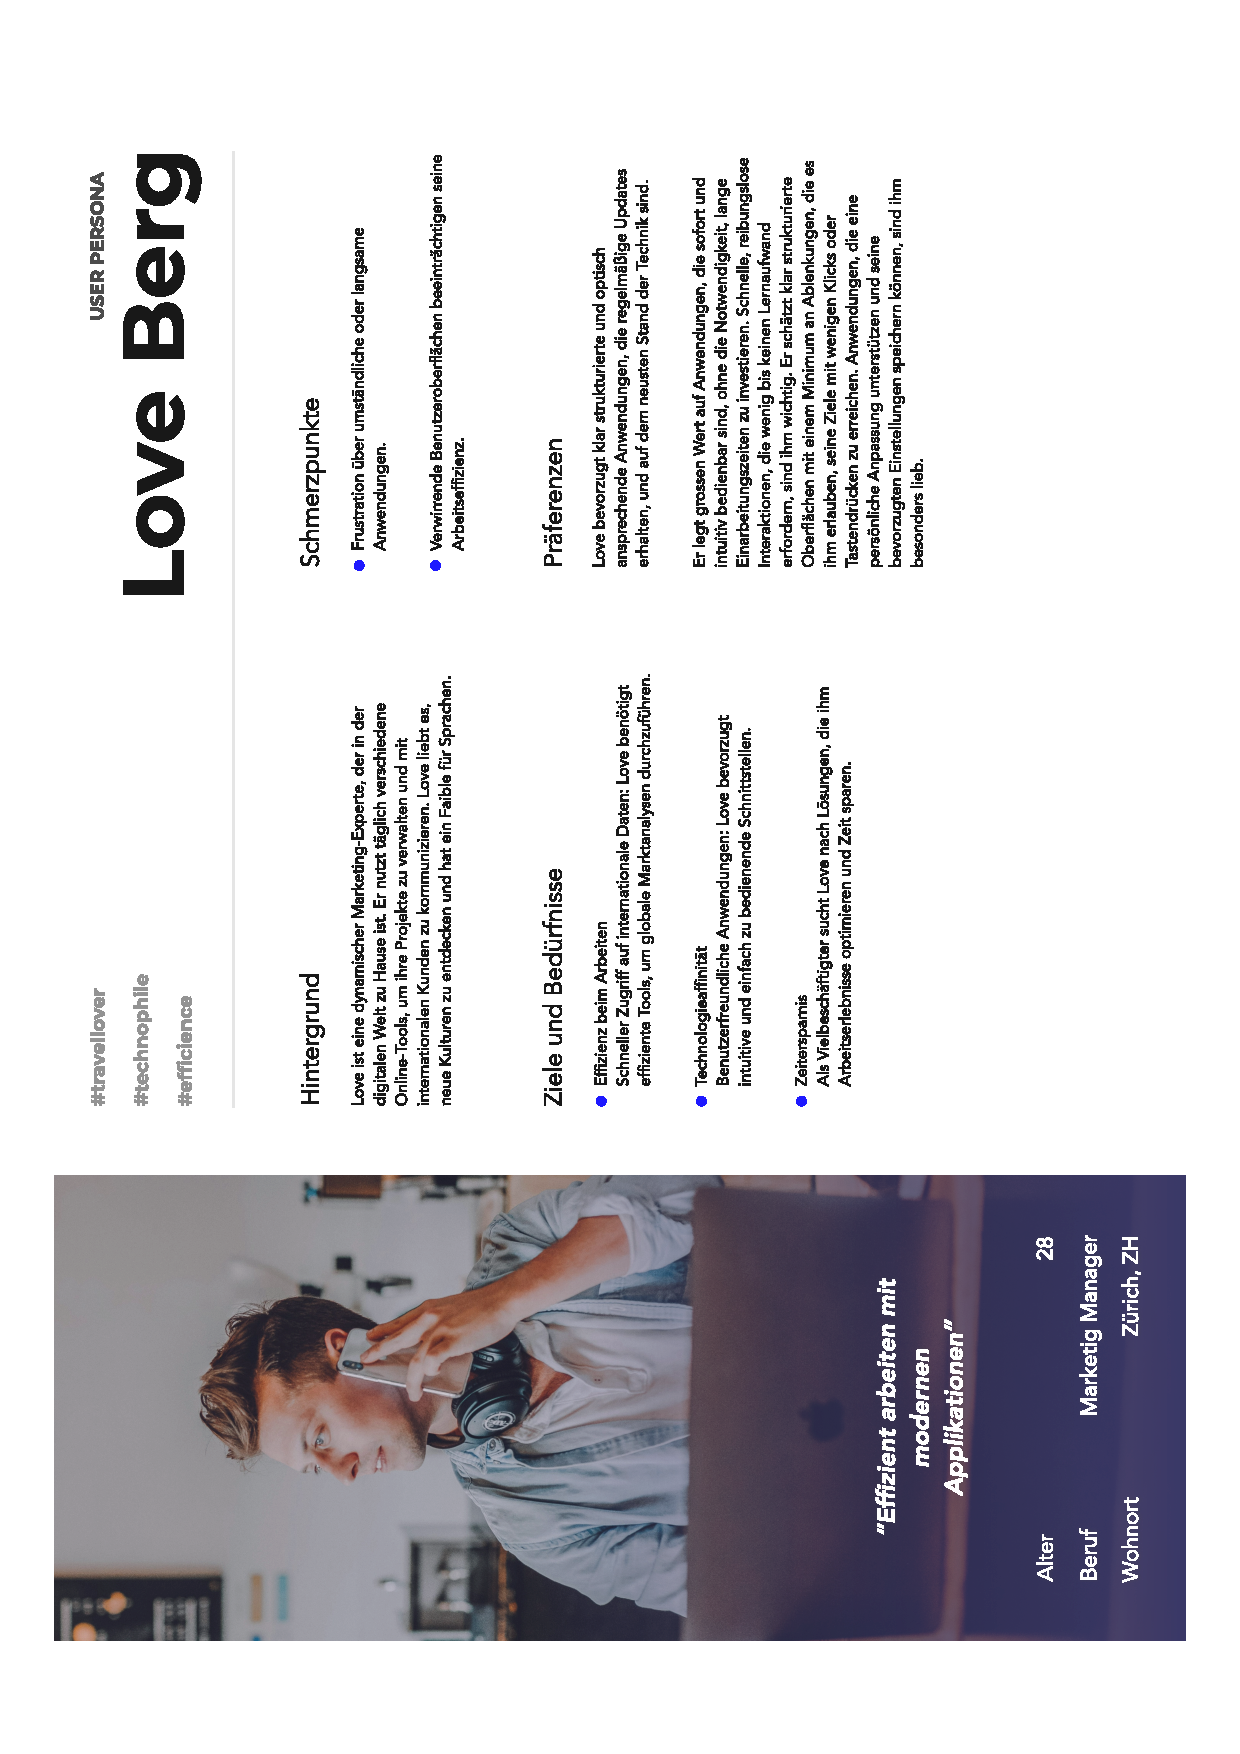
\includepdf[pages=-]{../appendix/Persona_User.pdf}
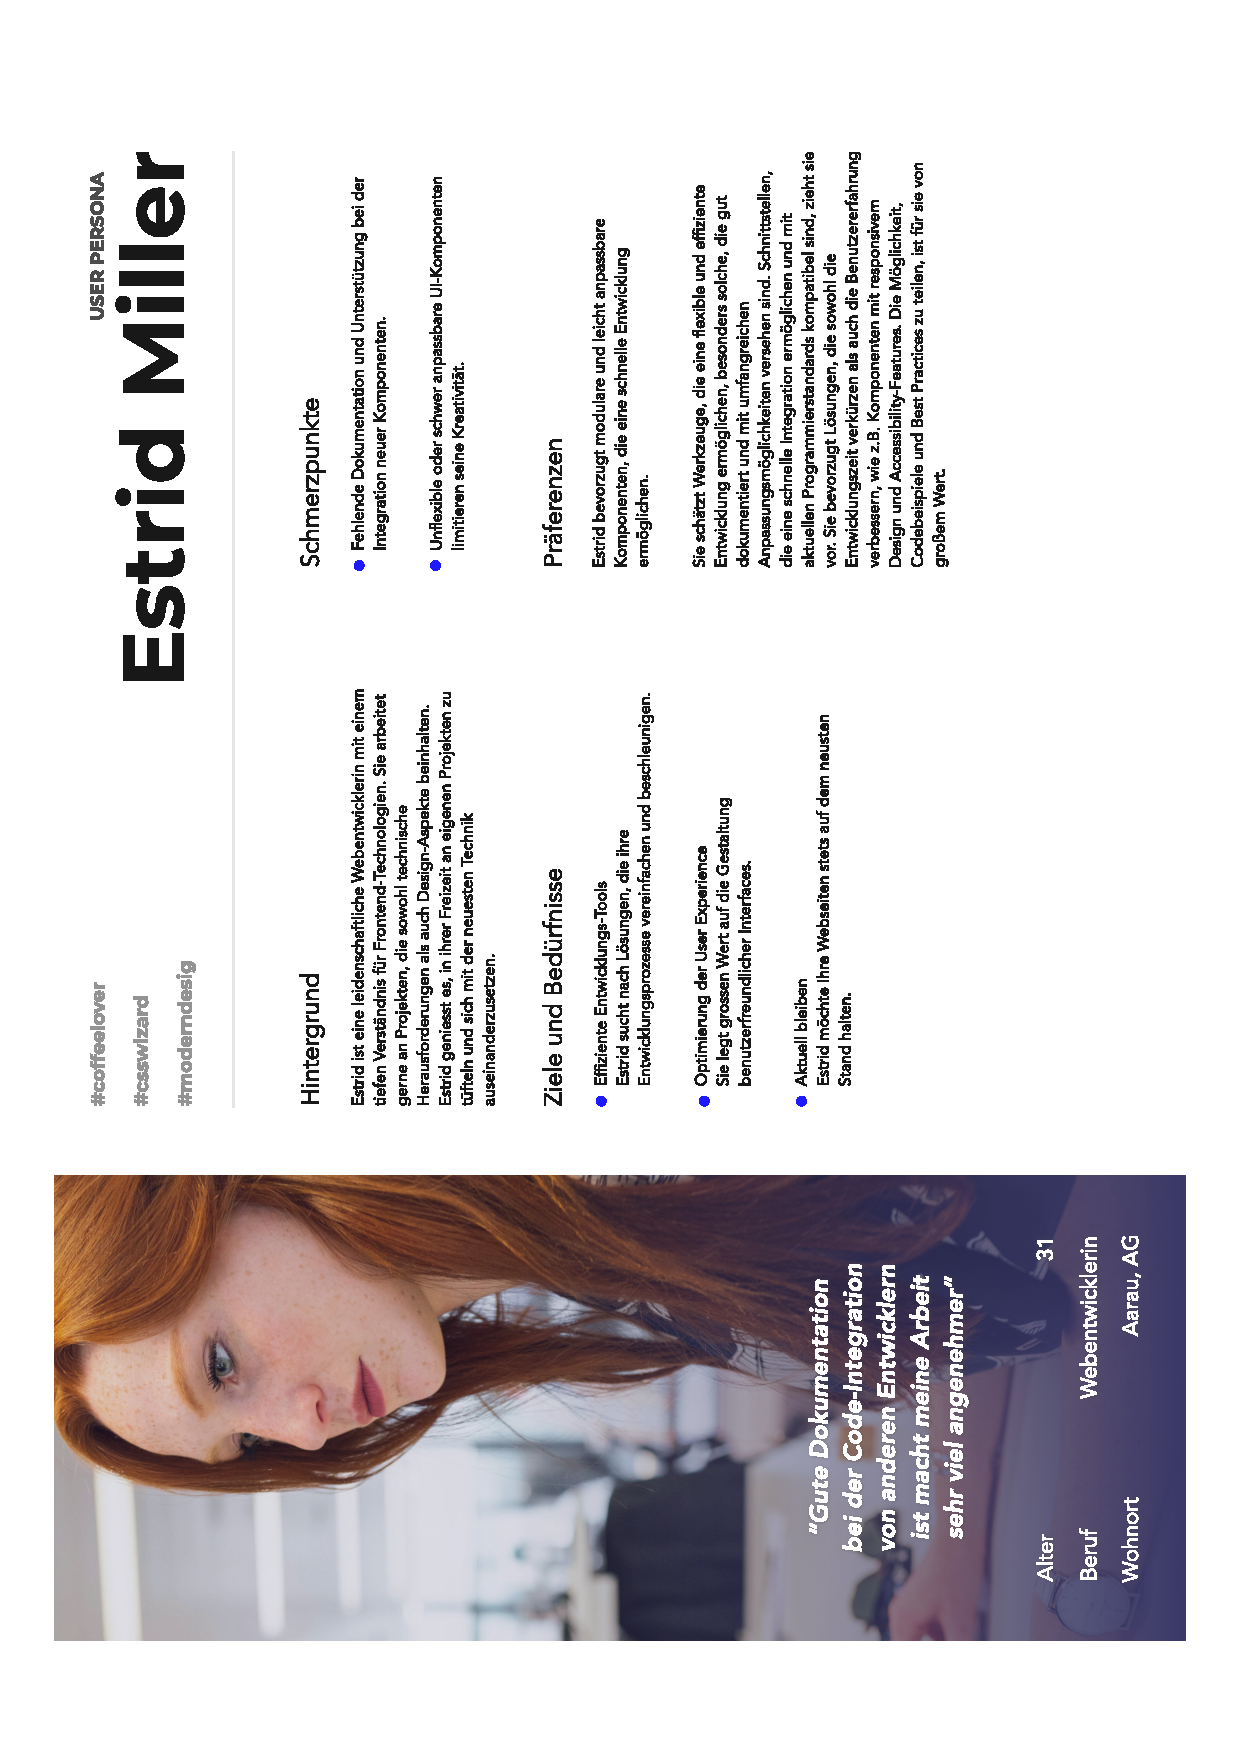
\includepdf[pages=-]{../appendix/Persona_Dev.pdf}



\chapter{Links}
\label{chap:links}

\begin{itemize}
    \item \textbf{Artefakte-Seite}: \burl{https://fhnw-ramonamarti.github.io/ip6/index.html}
    \item \textbf{Repository}: Projekt-Ordner 
        \begin{itemize}
            \item \textbf{Komponente}: \burl{https://github.com/fhnw-ramonamarti/Kolibri/tree/interactionLetters/docs/src/kolibri/projector/selectComponent}
            \item \textbf{Beispiele}: \burl{https://github.com/fhnw-ramonamarti/Kolibri/tree/interactionLetters/docs/src/examples/selectComponent}
        \end{itemize}
\end{itemize}



\chapter{API} % todo write api for usage component
\label{chap:api}

\import{../appendix}{api.tex}
